\section{Evaluation: Applications of \MLIR}

\MLIR is a system that aims to generalize and drive a wide range of
compiler projects, so our primary evaluation metric is to show that it
is being adopted and used for diverse projects.  We provide a summary
of community activity and describe a few use cases in more detail to
highlight the generality and extensibility of \MLIR and demonstrate
how well it implements the customizability design principle.

Today, \MLIR is a growing open source project with a community
spanning academia and industry.  For example, the academic workshop
about use of \MLIR in High-Performance Computing (HPC) was attended by
individuals from 16 universities and involved 4 national laboratories
from 4 different countries.  \MLIR was also endorsed by 14
multinational companies and at the LLVM Developer Meeting more than
100 industry developers attended a roundtable event about \MLIR.
Community adoption and participation is a proxy measure for usability
and need.  More than 26 dialects are in development in public or
private and 7 projects across different companies are replacing custom
infrastructure with \MLIR.  We argue that this shows a real need for
\MLIR, as well as endorses its usability.

\subsection{TensorFlow graphs}

While the other discussed representations are familiar to most compiler developments,
one of key use cases for \MLIR is to support the development of machine
learning frameworks. Their internal representations is often based on a data
flow graph~\cite{veen} with a dynamic execution semantics.

TensorFlow~\cite{tensorflow2015-whitepaper} is an example of such framework.
Its representation is a high-level dataflow computation where the
nodes are computations which can be placed on various devices, including
specific hardware accelerators.

\MLIR is used in TensorFlow to model this internal representation and perform
transformations for the use cases presented in \figref{ml-compile}: from
simple algebraic optimizations to retargeting graphs
for parallel execution on data center clusters of hardware accelerators, from
lowering to a representation suitable for mobile deployment to
generating efficient native code using tools like XLA~\cite{xla}. The representation of
a TensorFlow graph in \MLIR is illustrated on~\figref{tf}.

\begin{figure}[t]
  \centering
  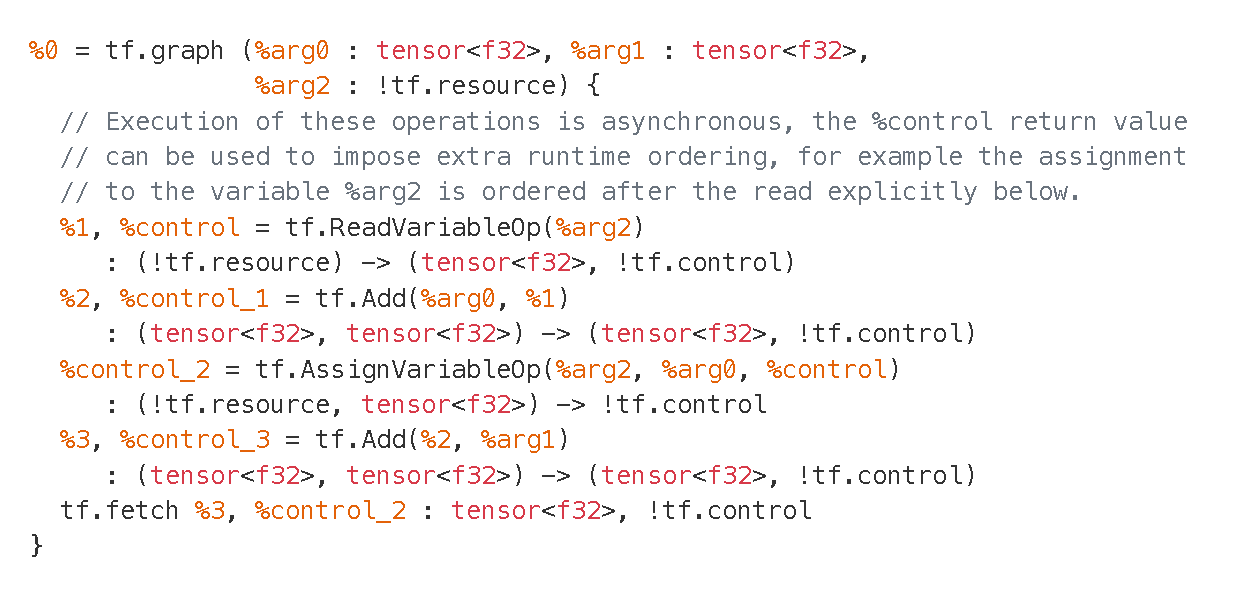
\includegraphics[width=.8\textwidth]{img/tf_mlir.pdf}
%\begin{tabular}{c}
%\begin{lstlisting}[language=mlir]
%%0 = tf.graph (%arg0 : tensor<f32>, %arg1 : tensor<f32>,
%               %arg2 : !tf.resource) {
% // Execution of these operations is asynchronous, the %control
% // return value can be used to impose extra runtime ordering,
% // for example the assignment to the variable %arg2 is ordered
% // after the read explicitly below.
% %1, %control = tf.ReadVariableOp(%arg2)
%     : (!tf.resource) -> (tensor<f32>, !tf.control)
% %2, %control_1 = tf.Add(%arg0, %1)
%     : (tensor<f32>, tensor<f32>) -> (tensor<f32>, !tf.control)
% %control_2 = tf.AssignVariableOp(%arg2, %2, %control)
%     : (!tf.resource, tensor<f32>) -> !tf.control
% %3, %control_3 = tf.Add(%2, %arg1)
%     : (tensor<f32>, tensor<f32>) -> (tensor<f32>, !tf.control)
% tf.fetch %3, %control_2 : tensor<f32>, !tf.control
%}
%
%\end{lstlisting}
%\end{tabular}
\caption{SSA representation of a TensorFlow dataflow graph in \MLIR.}\label{fig:tf}
\end{figure}


\subsection{Polyhedral code generation}\label{sec:affine}

One of the original motivations for \MLIR was the exploration of
polyhedral code generation for accelerators.
The affine dialect is a simplified polyhedral representation that was
designed to enable progressive lowering.
While a full exploration of the design points here is out of scope for this
paper, we illustrate aspects of the affine dialect to show the modeling power
of \MLIR and contrast the affine dialect with past
representations~\cite{Fea92b,uruk,isl,ppcg,tc}.

\subsubsection{Similarities}
The \MLIR affine dialect operates on a structured multi-dimensional
type for all accesses to memory.  In the default case, these structured types
are \emph{injective}: different indexings are guaranteed not to alias by
construction, a common precondition for polyhedral dependence analyses.

Affine modeling is split in two parts. Attributes are used to model affine
maps and integer sets at compile-time and Ops are used to apply affine
restrictions to the code. Namely, \lstinline|affine.for| Op is a ``for'' loop
with bounds expressed as affine maps of values required to be invariant in a
function. Thus loops have static control flow. Similarly,
\lstinline|affine.if| is a conditional restricted by affine integer sets.  The
bodies of loops and conditionals are regions that use \lstinline|affine.load|
and \lstinline|affine.store| to restrict indexing to affine forms of
surrounding loop iterators. This enables exact affine dependence analysis while
avoiding the need to infer affine forms from a lossy lower-level representation.

\begin{figure}[t]
  \centering
  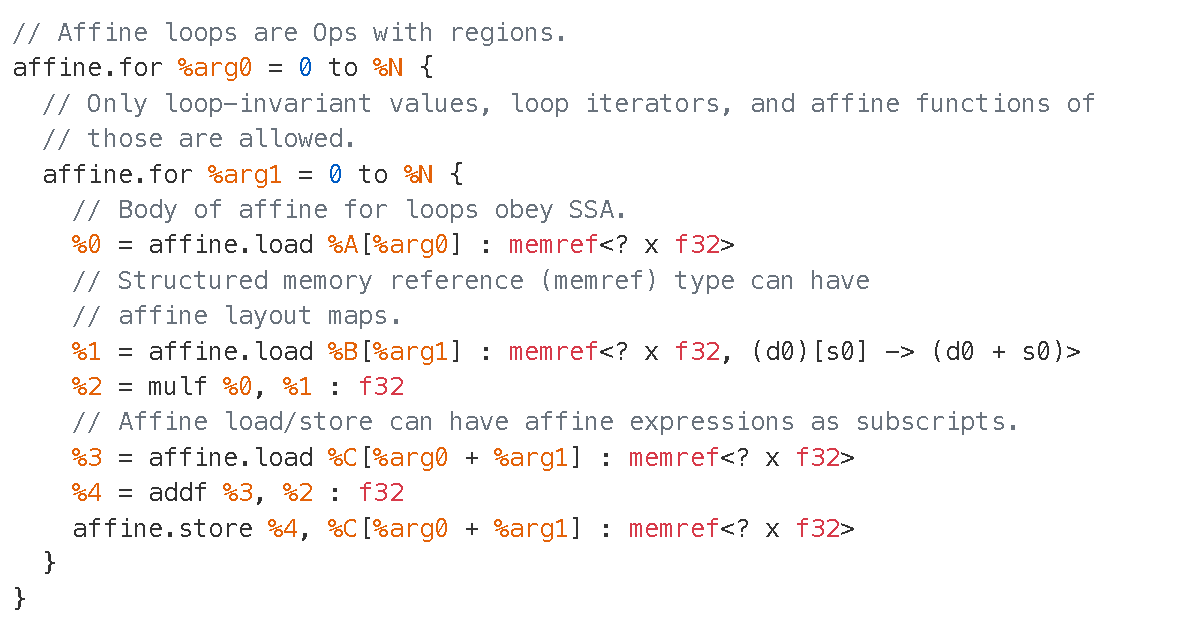
\includegraphics[width=.8\textwidth]{img/affine_mlir.pdf}
%  \lstinputlisting[language=mlir]{affine.mlir}
  \caption{Representing polynomial multiplication kernel
    \lstinline|C(i+j) += A(i) * B(j)| using \MLIR affine dialect.}
  \label{fig:affine}
\end{figure}

\subsubsection{Differences}
The differences with existing polyhedral frameworks are numerous, we can
characterize them in four categories:

(1) \emph{Rich types}: the \MLIR structured memory reference type contains a layout
map connecting the index space of the buffer to the actual address space.
This separation of concerns makes loop and data transformations compose better:
changes to data layout do not affect the code and do not pollute dependence
analysis. Such mixes of transformations have been explored
previously~\cite{chandan} but are uncommon.

(2) \emph{Mix of abstractions}: Bodies of affine loops in \MLIR can be expressed with
operations on typed SSA values.
Therefore, all traditional compiler analyses and transformations
remain applicable and can be interleaved with polyhedral transformations.  On
the contrary, polyhedral compilers often abstract such details away completely,
making it challenging for a polyhedral compiler to manipulate, e.g., vector
types.

(3) \emph{Smaller representation gap}: One of the key features of the polyhedral
model is its ability to represent the
order of loop iterations in the \emph{type system}. In this system, a large
number of loop transformations compose directly and can be reasoned about using
simple mathematical abstractions~\cite{uruk}. However, polyhedral
transformations require \emph{raising} into a representation often
drastically different from the original~\cite{polly,pollytactics}. Furthermore,
the conversion from
transformed polyhedra to loops is computationally hard~\cite{cloog}.
\MLIR-based representation maintains high-level loop structure around
lower-level representation, removing the need for raising.

(4) Compilation speed is a crucial goal for \MLIR as discussed in
\secref{parallel_comp}, but has not been a focus of most existing polyhedral
approaches.  These rely heavily on algorithms with exponential complexity: on integer
linear programming to derive loop orderings automatically and on polyhedron
scanning algorithms to convert the representation back to loops.
The approach taken by \MLIR explicitly does not rely on polyhedron scanning
since loops are preserved in the IR.

Experience with the affine dialect shows that it is useful for a wide range
of code generation projects, and its development was important exploration
that the \MLIR design made practical.

\iffalse
 A direct
consequence is that affine constructs are modeled as operations with special
semantics as described in 
\az{@ntv this must be finished}

Let us discuss several polyhedral representations. First algorithms by
Feautrier used multi-dimensional affine functions to express iteration
order~\cite{Fea92b}. The URUK framework separated the ordering between
individual loop iterations from the statement and loop ordering, which enabled
more declarative description of transformations and exploited the syntactic
structure to reduce the complexity of code generation~\cite{urgent}. Schedule
tree representation was driven by the GPU code generation needs
\az{cite Tobias Toplas}
and captures syntax-level ordering in an explicit tree structure
\az{cite Sven Impact}.
One can observe a trend towards including more of traditional compiler concepts
into polyhedral representations, partially attributable to the need for
mainstream adoption for polyhedral techniques.

\MLIR takes this integration further using the actual IR structure to represent
structural concepts, such as loop as branches, and by keeping most information
at the SSA value level, i.e. lifting everything into the type system.

\az{We need an actual description of how we encode polyhedral using IR
concepts, preferably before the discussion because the paper is about encoding
representations.}
For instance, the `affine.for` loop is still a higher-level type than
control-flow over basic blocks and generic `for` loops but does not have a
notion of iteration order. An `affine.for` loop produces an SSA-value for its
induction variable, that becomes a basic-block argument to the nested region.

\az{Etc describe affine in \MLIR, lift some example/desc from doc.}


%\subsubsection{Affine transformations}
%\TODO{do we want this?}
%
%\begin{figure}
%    \centering
%    %%\includegraphics{}
%    \caption{SGEMM performance comparison between code generated from affine dialect vs existing solutions.}
%    \label{fig:sgemm-results}
%\end{figure}

\fi

\subsection{Fortran IR (FIR)}

The LLVM Fortran frontend ``flang'' is currently under major development,
led by NVIDIA/PGI. Similar to Swift, Rust, and others, flang needs
a specialized IR in order to support advanced transformations
for high-performance Fortran codebase, and is using \MLIR to support
these Fortran-specific optimizations~\cite{flang}.  These high-level
optimizations---advanced loop
optimizations, array copy elimination, call specialization,
devirtualization---would be hard implement using only LLVM.

For example, FIR is able to model Fortran virtual dispatch table as a first
class concept (see~\figref{fir}).

\begin{figure}[h]
  \centering
  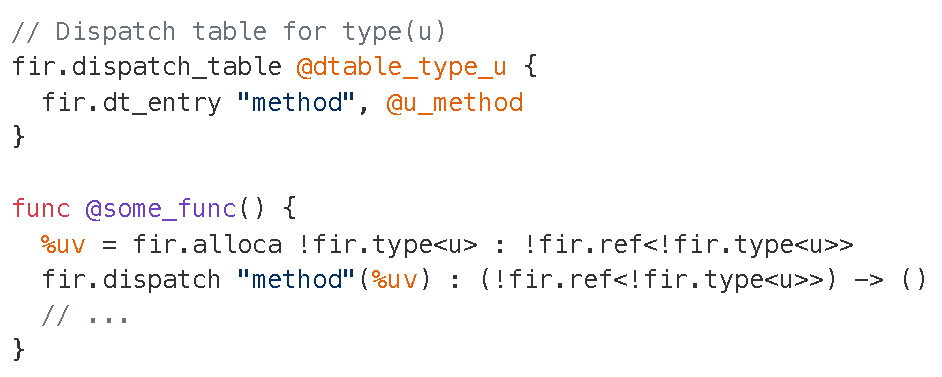
\includegraphics[width=.7\textwidth]{img/flang_mlir.pdf}
%\begin{tabular}{c}
%\begin{lstlisting}[language=mlir]
%// Dispatch table for type(u)
%fir.dispatch_table @dtable_type_u {
%  fir.dt_entry "method", @u_method
%}
%
%func @some_func() {
%  %uv = fir.alloca !fir.type<u> : !fir.ref<!fir.type<u>>
%  fir.dispatch "method"(%uv) : (!fir.ref<!fir.type<u>>) -> ()
%  // ...
%}
%\end{lstlisting}
%\end{tabular}

\caption{FIR has first class support for dynamic virtual function
dispatch table.}\label{fig:fir}
\end{figure}

The ability to model the high-level semantics of the programming language in a
structured IR is very powerful. For example, first-class modeling of the
dispatch tables allows a robust devirtualization pass to be implemented.  While
this could have been implemented with a bespoke compiler IR, the
use of \MLIR allowed the flang developers to spend their engineering resources
focused on the IR design for their domain instead of reimplementing basic
infrastructure.

The choice of \MLIR also unlocks the reusability of other dialects that are not
specific to Fortran: a language-independent OpenMP dialect could be shared
between Fortran and C language frontends.  Similarly, targeting a
heterogeneous platform using OpenACC
becomes tractable within \MLIR through the sharing and reuse of the
GPU-oriented dialects and passes. This is straightforward thanks to \MLIR 
begin specifically designed to support a mix of composable dialects.



\subsection{Domain-specific compilers}

The applications of \MLIR above are within large compilation
workflows, but it is also used to build domain specific compilers for
specific small workflows.  A reusable and modular infrastructure makes
these specialized paths feasible and relatively cheap to build.

\paragraph{Optimizing \MLIR pattern rewriting}

\MLIR has an extensible system for pattern rewrites described in~\secref{infra}.
In addition to statically declared patterns, we had
applications where the rewrite patterns needed to be dynamically
extensible at runtime, allowing hardware vendors to add new lowerings
in drivers.  The solution was to express \MLIR pattern rewrites as an
\MLIR dialect itself, allowing us to use \MLIR infrastructure to build
and optimize efficient Finite State Machine (FSM) matcher and
rewriters on the fly.  This work includes FSM optimizations seen in
other systems, such as the LLVM SelectionDAG and GlobalISel
instruction selection systems.

%\paragraph{Scientific modeling abstractions}
%	Domain specific dialect for scientific modeling, in particular dialect created for
%  weather modeling, is being developed. This dialect, combined with another intermediate dialect,
%  allows specifying the simulation problem at a high level, optimizing at the
%  domain specific levels before lowering to affine and finally code generation.

\paragraph{Lattice regression compiler}

Lattice regression~\cite{NIPS2009_3694} is a machine learning
technique renowned for fast evaluation times and interpretability.
The predecessor of the compiler was implemented using \Cpp
templates. This allowed for high-performance code with
metaprogramming, but expressing general optimizations on the
end-to-end models was not straightforward. This particular lattice
regression system is used in applications with multiple millions of
users and hence performance improvements are critical.

\MLIR was used as the basis for a new compiler for this specialized
area, which was driven by a specialized search approach---effectively
resulting in a machine learning problem being solved during
compilation. The resultant compiler was developed by investing a  3
person-month effort, and resulted in up to $8\times$ performance improvement
on a production model, while also improving transparency during
compilation.
